%!TEX program = xelatex
\documentclass{article}
\usepackage[
  a4paper,
  top=3cm,
  bottom=3cm,
  left=2cm,
  right=2cm
]{geometry}
\usepackage{ctex}
\usepackage{graphicx}
\usepackage{amsmath}
\usepackage{siunitx}
\usepackage{listingsutf8}
\title{超静定梁塑性极限分析}
\author{王勇 wangyong.seu@qq.com}
\begin{document}
\maketitle
\section{问题描述}
一矩形截面超静定梁,基本布置如图\ref{fig:beam-diagram}所示。
梁长\SI{5}{m},截面高\SI{0.2}{m},宽\SI{0.1}{m}。
材料弹性模量$E=\SI{2.0E5}{MPa}$,泊松比$\mu=0.2$,按理想弹塑性考虑,材料屈服强度为$\SI{335}{MPa}$,跨中作用一个集中荷载$P$。
试分析超静定梁的极限承载力大小。

\begin{figure}[!h]
\centering
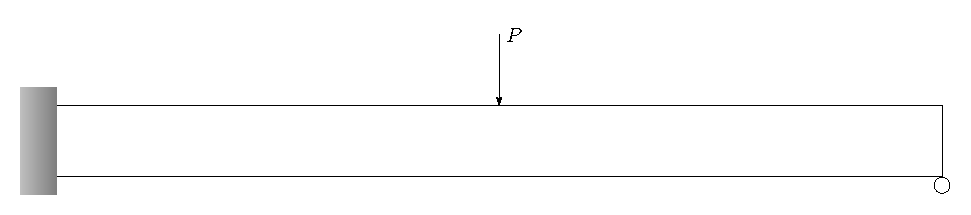
\includegraphics[width=0.6\textwidth]{beam_diagram.pdf}
\caption{超静定梁示意图}\label{fig:beam-diagram}
\end{figure}

\section{解题思路}
本例需要进行弹塑性分析,故使用BEAM189单元模拟超静定梁。
材料本构关系采用双折线随动强化模型BKIN进行模拟。
左端约束所有方向自由度,右侧约束$x$和$y$向平动自由度,在跨中施加集中力。

\end{document}